%**************************************************************************************
\section{Phenomenology and Modeling of Bottom Reflood}\label{sec:reflood_phenomenology}
%**************************************************************************************

% Opening Paragraph
% Why Reflood is important, what is reflood, how does the cladding temperature behaves typically

% The phenomenology
% What kind of flow regime is observed

% FEBA Test No. 216 Prior Uncertainty Propagation, DP
\begin{figure}[bth]
    \centering
    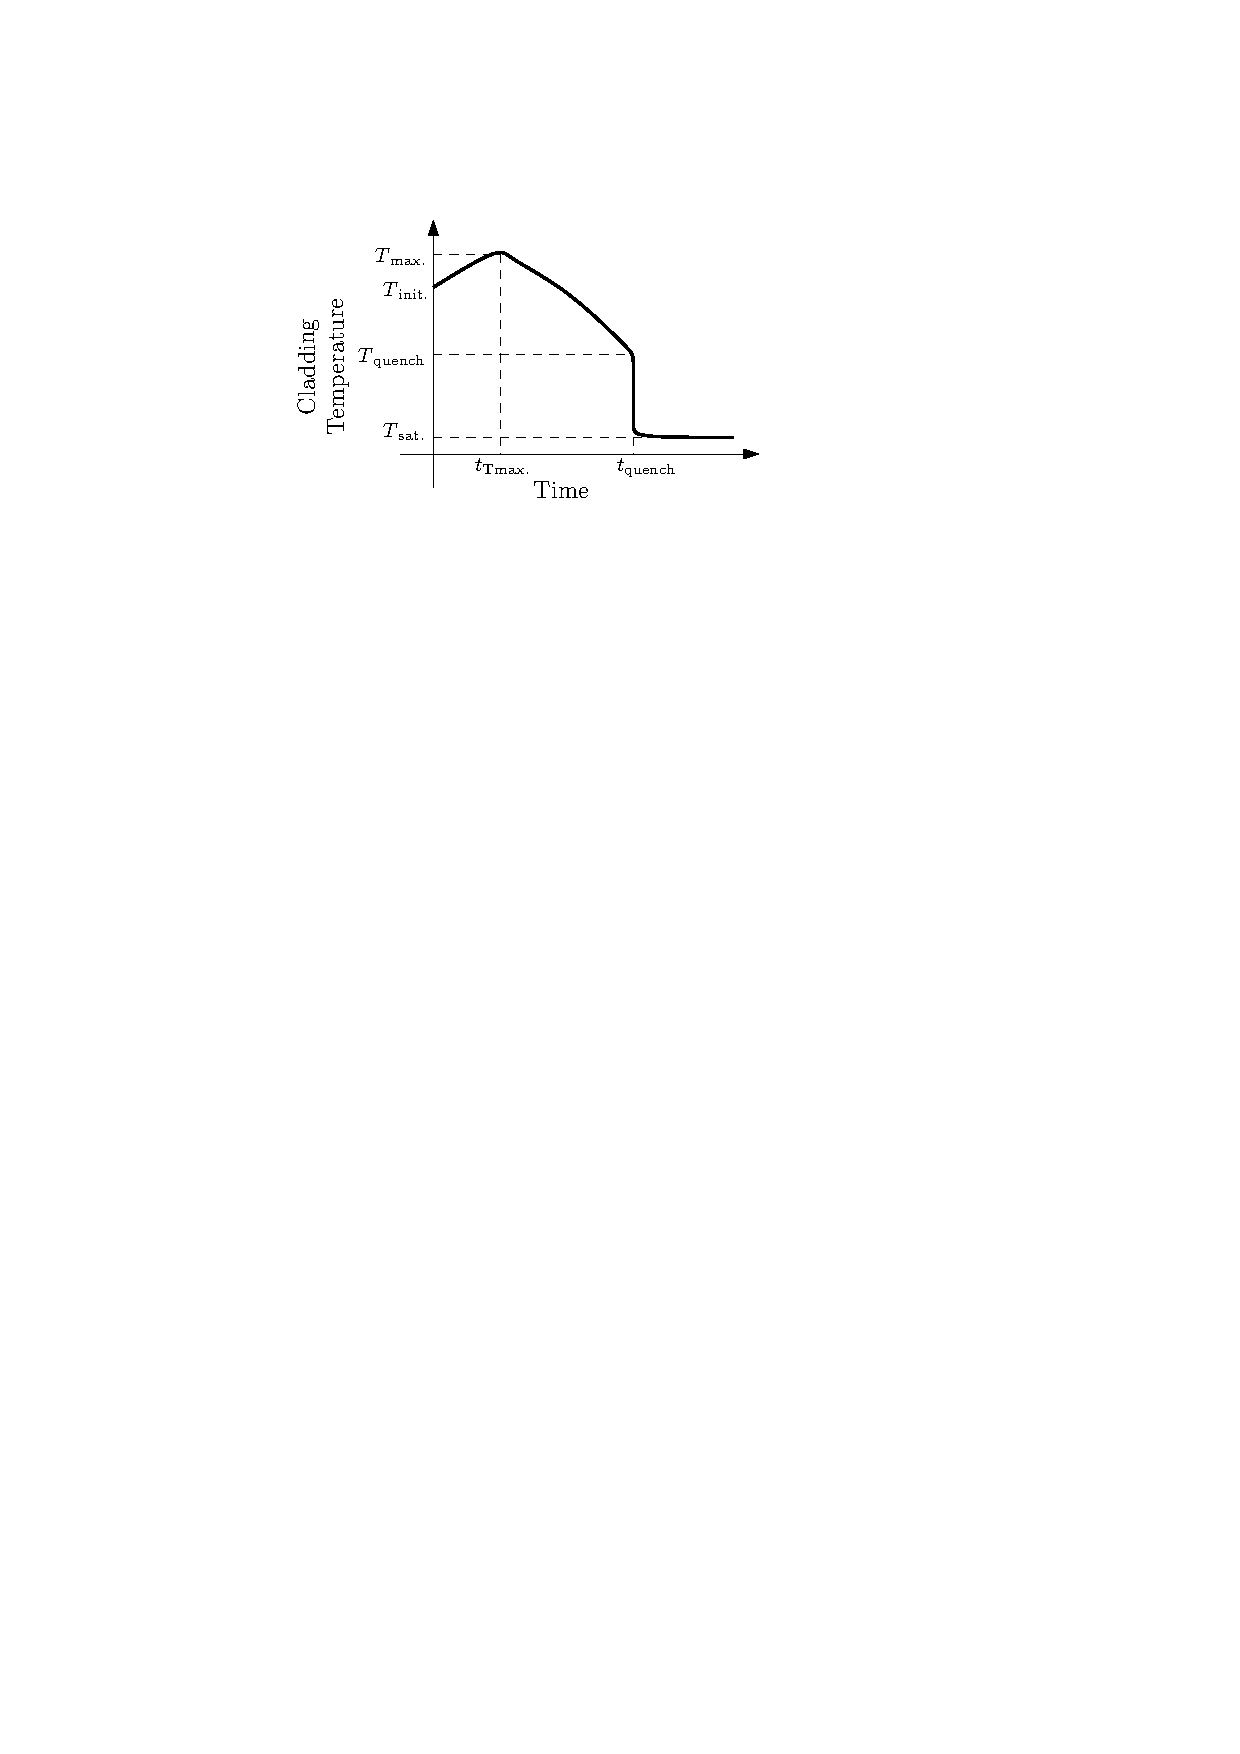
\includegraphics[width=1.0\textwidth]{../figures/chapter2/figures/refloodCurveQoIs}
    \caption[A typical cladding temperature evolution during constant flooding rate reflooding at mid-height assembly.]{A typical cladding temperature evolution during constant flooding rate reflooding at mid-height assembly (adapted from \cite{Zeng2010}). The labels on the both axes are typical \glspl[hyper=false]{qoi} of reflood transient, where the abbreviations $max.$, $init.$, and $sat.$ refer to the \emph{maximum}, \emph{initial}, and \emph{saturation}, respectively.}
    \label{fig:ch2_reflood_curve_qois}
\end{figure}

% The Modeling of The Phenomenology
\normdoublefigure[pos=tbhp,
                  mainlabel={fig:ch2_reflood_phenomenology},
                  maincaption={Phenomenology of flow during reflood according to \gls[hyper=false]{trace} code and the corresponding .},
				mainshortcaption={Phenomenology of flow during reflood according to \gls[hyper=false]{trace} code.},
                  leftopt={width=0.45\textwidth},
                  leftlabel={fig:ch2_reflood_curve_phenomenology},
                  leftcaption={post-\gls[hyper=false]{chf} flow regimes $(2)$--$(5)$},
                  %leftshortcaption={},%
                  rightopt={width=0.5\textwidth},
                  rightlabel={fig:ch2_post_chf_regime},
                  rightcaption={Reflood curve}]
{../figures/chapter2/figures/postCHFRegime}
{../figures/chapter2/figures/refloodCurvePhenomenology}
